\documentclass[12pt,a4paper,oneside]{article}

\usepackage[utf8]{inputenc}
\usepackage[portuguese]{babel}
\usepackage[T1]{fontenc}
\usepackage{amsmath}
\usepackage{amsfonts}
\usepackage{amssymb}
\usepackage{graphicx}

\usepackage{xcolor}
% Definindo novas cores
\definecolor{verde}{rgb}{0.25,0.5,0.35}
\definecolor{jpurple}{rgb}{0.5,0,0.35}
% Configurando layout para mostrar codigos Java
\usepackage{listings}
\lstset{
  language=Java,
  basicstyle=\ttfamily\small, 
  keywordstyle=\color{jpurple}\bfseries,
  stringstyle=\color{red},
  commentstyle=\color{verde},
  morecomment=[s][\color{blue}]{/**}{*/},
  extendedchars=true, 
  showspaces=false, 
  showstringspaces=false, 
  numbers=left,
  numberstyle=\tiny,
  breaklines=true, 
  backgroundcolor=\color{cyan!10}, 
  breakautoindent=true, 
  captionpos=b,
  xleftmargin=0pt,
  tabsize=4,
  escapeinside=||
}

\author{\\Universidade Federal de Goiás (UFG) - Regional Jataí\\Bacharelado em Ciência da Computação \\Teoria de Grafos \\Esdras Lins Bispo Jr.}

\title{\sc \huge Prova (Parte 1)}

\date{29 de agosto de 2017}

\begin{document}

\maketitle

{\bf ORIENTAÇÕES PARA A RESOLUÇÃO}

\footnotesize

\begin{itemize}
	\item A avaliação é individual, sem consulta;
	\item A pontuação máxima desta avaliação é 10,0 (dez) pontos, sendo uma das 06 (seis) componentes que formarão a média final da disciplina: quatro testes, uma prova e os exercícios de aquecimento;
	\item A média final ($MF$) será calculada assim como se segue
	\begin{eqnarray}
		MF & = & MIN(10, S) \nonumber \\
		S & = & (\sum_{i=1}^{4} 0,2.T_i ) + 0,2.P  + 0,1.EA \nonumber
	\end{eqnarray}
	em que 
	\begin{itemize}
		\item $S$ é o somatório da pontuação de todas as avaliações,
		\item $T_i$ é a pontuação obtida no teste $i$,
		\item $P$ é a pontuação obtida na prova, e
		\item $EA$ é a pontuação total dos exercícios de aquecimento.
	\end{itemize}
	\item O conteúdo exigido compreende os seguintes pontos apresentados no Plano de Ensino da disciplina: (1) Noções Básicas de Grafos, (2) Caminhos e Circuitos, e (3) Subgrafos.
\end{itemize}


\begin{center}
	\fbox{\large Nome: \hspace{10cm}}
	\fbox{\large Assinatura: \hspace{9cm}}
\end{center}

\newpage

\normalsize

\begin{enumerate}
	
	\section*{Primeiro Teste}
	
	\item (5,0 pt) {\bf [E 1.14]} Para qualquer inteiro positivo $k$, um cubo de dimensão $k$ (ou $k$-cubo) é o grafo definido da seguinte maneira: os vértices do grafo são todas as sequências $b_1 b_2 \ldots b_k$ de bits; dois vértices são adjacentes se e somente se
	diferem em exatamente uma posição. Por exemplo, os vértices do cubo de dimensão 3 são 000, 001, 010, 011, 100, 101, 110, 111; o vértice 000 é adjacente aos vértices 001, 010, 100 e a nenhum outro; e assim por diante. O cubo de dimensão $k$ será denotado por $Q_k$.
	\begin{enumerate}
		\item (2,0 pt) Faça figuras dos cubos $Q_1$, $Q_2$ e $Q_3$.
		
		\vspace*{0.1cm} 
		
		{\color{blue} {\bf Resposta:} 
			\begin{flushleft}
				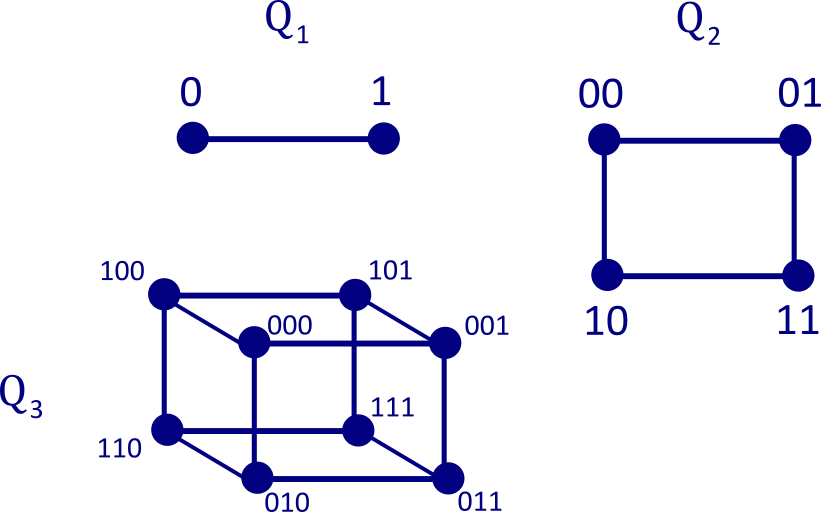
\includegraphics[width=0.7\textwidth]{images/cubos}
			\end{flushleft}
		}
		\item (1,5 pt) Quantos vértices tem $Q_k$? Justifique.
		
		\vspace*{0.1cm} 
		
		{\color{blue} {\bf Resposta:}
			Os vértices de um $Q_k$ são todas as sequências distintas de $k$ bits. Logo, aplicando o princípio multiplicativo, $Q_k$ tem $2^k$ vértices.
		} 
		\item (1,5 pt) Quantas arestas tem $Q_k$? Justifique.
		
		\vspace*{0.1cm} 
		
		{\color{blue} {\bf Resposta:}
			Todo grafo $r$-regular de $n$ vértices tem $rn/2$ arestas. Cada vértice $v$ de um $Q_k$ tem grau $k$. Isto é verdade, pois cada um de seus vizinhos tem apenas um bit distinto de $v$. Logo, o $Q_k$ é $k$-regular e tem $2^k \times (k/2)$ arestas.
		} 
	\end{enumerate}
	
	\newpage
	
	\item (5,0 pt) {\bf [E 1.33]} Se $G$ é um $K_n$, quanto valem $\delta(G)$ e $\Delta(G)$? \\Quanto valem os parâmetros $\delta$ e $\Delta$ de um $K_{p,q}$? Justifique sua resposta.
	
	\vspace*{0.1cm} 
	
	{\color{blue} {\bf Resposta:}
		Qualquer vértice de um $K_n$ tem $n-1$ vizinhos, i.e., o número máximo de vizinhos possível. Logo, se $G$ é um $K_n$, $\delta(G) = \Delta(G) = n-1$.
		
		Em um $K_{p.q}$, cada vértice branco tem $q$ vizinhos e cada vértice preto tem $p$ vizinhos. Logo, $\delta(K_{p,q}) = min(p,q)$ e $\Delta(K_{p,q}) = max(p,q)$.
	} 
	
	\section*{Segundo Teste}
	
	\item (5,0 pt) {\bf [E 1.29]} É verdade que o grafo do cavalo no tabuleiro $t$-por-$t$ é bipartido? Justifique sua resposta.
	
	\vspace*{0.1cm} 
	
	{\color{blue} {\bf Resposta:}
		É verdade para $t>1$. Para $t=1$, é impossível estabelecer uma bipartição nos vértices do grafo, pois é necessário que cada partição seja não-vazia.
		
		Entretanto, é possível estabelecer a bipartição para $t>1$. Basta representarmos os vértices pretos e brancos pelas casas pretas e brancas do tabuleiro, respectivamente. Desta forma, garantimos que qualquer aresta do grafo tem uma ponta branca e uma ponta preta. Isto é verdade, pois o cavalo estando em uma casa preta, só consegue mover-se para uma casa branca (e vice-versa). 
	} 
	
	\item (5,0 pt) {\bf [E 1.88]} Seja $G$ um grafo, $V'$ um subconjunto de $V_G$, e $E'$ um subconjunto de $E_G$. É verdade que $(V', E')$ é um subgrafo de $G$? Justifique sua resposta.
	
	\vspace*{0.1cm} 
	
	{\color{blue} {\bf Resposta:}
		Isto não é sempre verdade. Como contra-exemplo, pode-se mostrar o grafo $G = (V, E)$ em que $V = \{a, b, c\}$ e $E = \{ab\}$. Faça $V' = \{c\}$ e $E' = \{ab\}$. Garante-se que $V' \subseteq V$ e $E' \subseteq E$, mas $(V', E')$ não é um grafo e, por consequência, não é um subgrafo de $G$.
	} 
	
	\end{enumerate}
\end{document}